% Options for packages loaded elsewhere
% Options for packages loaded elsewhere
\PassOptionsToPackage{unicode}{hyperref}
\PassOptionsToPackage{hyphens}{url}
\PassOptionsToPackage{dvipsnames,svgnames,x11names}{xcolor}
%
\documentclass[
  a4paper,
  DIV=11,
  numbers=noendperiod,
  oneside]{scrreprt}
\usepackage{xcolor}
\usepackage{amsmath,amssymb}
\setcounter{secnumdepth}{5}
\usepackage{iftex}
\ifPDFTeX
  \usepackage[T1]{fontenc}
  \usepackage[utf8]{inputenc}
  \usepackage{textcomp} % provide euro and other symbols
\else % if luatex or xetex
  \usepackage{unicode-math} % this also loads fontspec
  \defaultfontfeatures{Scale=MatchLowercase}
  \defaultfontfeatures[\rmfamily]{Ligatures=TeX,Scale=1}
\fi
\usepackage{lmodern}
\ifPDFTeX\else
  % xetex/luatex font selection
\fi
% Use upquote if available, for straight quotes in verbatim environments
\IfFileExists{upquote.sty}{\usepackage{upquote}}{}
\IfFileExists{microtype.sty}{% use microtype if available
  \usepackage[]{microtype}
  \UseMicrotypeSet[protrusion]{basicmath} % disable protrusion for tt fonts
}{}
\makeatletter
\@ifundefined{KOMAClassName}{% if non-KOMA class
  \IfFileExists{parskip.sty}{%
    \usepackage{parskip}
  }{% else
    \setlength{\parindent}{0pt}
    \setlength{\parskip}{6pt plus 2pt minus 1pt}}
}{% if KOMA class
  \KOMAoptions{parskip=half}}
\makeatother
% Make \paragraph and \subparagraph free-standing
\makeatletter
\ifx\paragraph\undefined\else
  \let\oldparagraph\paragraph
  \renewcommand{\paragraph}{
    \@ifstar
      \xxxParagraphStar
      \xxxParagraphNoStar
  }
  \newcommand{\xxxParagraphStar}[1]{\oldparagraph*{#1}\mbox{}}
  \newcommand{\xxxParagraphNoStar}[1]{\oldparagraph{#1}\mbox{}}
\fi
\ifx\subparagraph\undefined\else
  \let\oldsubparagraph\subparagraph
  \renewcommand{\subparagraph}{
    \@ifstar
      \xxxSubParagraphStar
      \xxxSubParagraphNoStar
  }
  \newcommand{\xxxSubParagraphStar}[1]{\oldsubparagraph*{#1}\mbox{}}
  \newcommand{\xxxSubParagraphNoStar}[1]{\oldsubparagraph{#1}\mbox{}}
\fi
\makeatother


\usepackage{longtable,booktabs,array}
\usepackage{calc} % for calculating minipage widths
% Correct order of tables after \paragraph or \subparagraph
\usepackage{etoolbox}
\makeatletter
\patchcmd\longtable{\par}{\if@noskipsec\mbox{}\fi\par}{}{}
\makeatother
% Allow footnotes in longtable head/foot
\IfFileExists{footnotehyper.sty}{\usepackage{footnotehyper}}{\usepackage{footnote}}
\makesavenoteenv{longtable}
\usepackage{graphicx}
\makeatletter
\newsavebox\pandoc@box
\newcommand*\pandocbounded[1]{% scales image to fit in text height/width
  \sbox\pandoc@box{#1}%
  \Gscale@div\@tempa{\textheight}{\dimexpr\ht\pandoc@box+\dp\pandoc@box\relax}%
  \Gscale@div\@tempb{\linewidth}{\wd\pandoc@box}%
  \ifdim\@tempb\p@<\@tempa\p@\let\@tempa\@tempb\fi% select the smaller of both
  \ifdim\@tempa\p@<\p@\scalebox{\@tempa}{\usebox\pandoc@box}%
  \else\usebox{\pandoc@box}%
  \fi%
}
% Set default figure placement to htbp
\def\fps@figure{htbp}
\makeatother


% definitions for citeproc citations
\NewDocumentCommand\citeproctext{}{}
\NewDocumentCommand\citeproc{mm}{%
  \begingroup\def\citeproctext{#2}\cite{#1}\endgroup}
\makeatletter
 % allow citations to break across lines
 \let\@cite@ofmt\@firstofone
 % avoid brackets around text for \cite:
 \def\@biblabel#1{}
 \def\@cite#1#2{{#1\if@tempswa , #2\fi}}
\makeatother
\newlength{\cslhangindent}
\setlength{\cslhangindent}{1.5em}
\newlength{\csllabelwidth}
\setlength{\csllabelwidth}{3em}
\newenvironment{CSLReferences}[2] % #1 hanging-indent, #2 entry-spacing
 {\begin{list}{}{%
  \setlength{\itemindent}{0pt}
  \setlength{\leftmargin}{0pt}
  \setlength{\parsep}{0pt}
  % turn on hanging indent if param 1 is 1
  \ifodd #1
   \setlength{\leftmargin}{\cslhangindent}
   \setlength{\itemindent}{-1\cslhangindent}
  \fi
  % set entry spacing
  \setlength{\itemsep}{#2\baselineskip}}}
 {\end{list}}
\usepackage{calc}
\newcommand{\CSLBlock}[1]{\hfill\break\parbox[t]{\linewidth}{\strut\ignorespaces#1\strut}}
\newcommand{\CSLLeftMargin}[1]{\parbox[t]{\csllabelwidth}{\strut#1\strut}}
\newcommand{\CSLRightInline}[1]{\parbox[t]{\linewidth - \csllabelwidth}{\strut#1\strut}}
\newcommand{\CSLIndent}[1]{\hspace{\cslhangindent}#1}



\setlength{\emergencystretch}{3em} % prevent overfull lines

\providecommand{\tightlist}{%
  \setlength{\itemsep}{0pt}\setlength{\parskip}{0pt}}



 


\usepackage{unicode-math}%
\setmathfont{XITS Math}%
\usepackage{fontspec}%
\setmainfont[Ligatures ={Common, TeX}, Scale=1, RawFeature={+cpsp}]{XITS} 
%Numbers={Lining,Proportional},Ligatures ={Common, TeX},RawFeature={+tnum,+cpsp,+frac},
\setsansfont[RawFeature={+cpsp},Scale=MatchLowercase]{Helvetica Neue}%
\setmonofont[Scale=0.78]{MesloLGS NF}%

\usepackage[a4paper,%
margin=2.5cm,%
bottom=3cm,%
top=3cm]{geometry}%
\usepackage{afterpage}% for "\afterpage"
\usepackage{xcolor}%
\definecolor{dundeeblue}{HTML}{4365E2}%
\usepackage{pagecolor}% With option pagecolor={somecolor or none}
%% For nice tables
\usepackage{booktabs}%
\usepackage{longtable}%
\usepackage{array}%
\usepackage{multirow}%
\usepackage{wrapfig}%
\usepackage{float}%
\usepackage{colortbl}%
\usepackage{pdflscape}%
\usepackage{tabu}%
%\usepackage{threeparttable}%
%\usepackage{threeparttablex}%
%\usepackage[normalem]{ulem}%
\usepackage{makecell}%
%% Wrap long output lines
\usepackage{listings}%
\lstset{breaklines=true}%
\usepackage{enumitem}%
\setlist[description]{style=nextline}%
%% For nice info boxes
\usepackage{fontawesome5}%
\usepackage{awesomebox}%
\usepackage{siunitx}%
\newcolumntype{d}{S[table-format=3.2]}%
\renewcommand{\bibname}{References}%
%\usepackage[colorlinks]{hyperref}%

\usepackage{titling}%
%\setlength{\droptitle}{8cm}
\pretitle{\newpagecolor{dundeeblue}\afterpage{\restorepagecolor} \vfill \begin{flushleft}
\fontsize{68pt}{62pt} \color{white}\sffamily\bfseries\selectfont }
\posttitle{\end{flushleft}}

\preauthor{\vspace{2.5cm} \begin{flushleft} \fontsize{18pt}{14pt} \color{white}\sffamily\selectfont}
\postauthor{$\quad\bullet\quad$ehall001@dundee.ac.uk\end{flushleft}}

\predate{\begin{flushleft} \fontsize{18pt}{14pt} \color{white}\sffamily\selectfont}
\postdate{\\ \vspace{1cm}
\includegraphics[width=10cm]{assets/images/rev_logo.pdf}\end{flushleft}}

%%% BEGIN SHORTCUTS
\DeclareMathOperator{\E}{\mathbf{E}}%
\DeclareMathOperator{\Var}{Var}%
\DeclareMathOperator{\Cov}{Cov}%
\DeclareMathOperator{\corr}{corr}%
\DeclareMathOperator{\sd}{sd}%
\newcommand{\se}{\mathsf{se}}%
%%% END SHORTCUTS

%% Change chapter to Topic
\makeatletter
\renewcommand{\@chapapp}{Topic}
\makeatother

\usepackage{tocbibind}



\usepackage{booktabs}
\usepackage{longtable}
\usepackage{array}
\usepackage{multirow}
\usepackage{wrapfig}
\usepackage{float}
\usepackage{colortbl}
\usepackage{pdflscape}
\usepackage{tabu}
\usepackage{threeparttable}
\usepackage{threeparttablex}
\usepackage[normalem]{ulem}
\usepackage{makecell}
\usepackage{xcolor}
\KOMAoption{captions}{tableheading}
\makeatletter
\@ifpackageloaded{tcolorbox}{}{\usepackage[skins,breakable]{tcolorbox}}
\@ifpackageloaded{fontawesome5}{}{\usepackage{fontawesome5}}
\definecolor{quarto-callout-color}{HTML}{909090}
\definecolor{quarto-callout-note-color}{HTML}{0758E5}
\definecolor{quarto-callout-important-color}{HTML}{CC1914}
\definecolor{quarto-callout-warning-color}{HTML}{EB9113}
\definecolor{quarto-callout-tip-color}{HTML}{00A047}
\definecolor{quarto-callout-caution-color}{HTML}{FC5300}
\definecolor{quarto-callout-color-frame}{HTML}{acacac}
\definecolor{quarto-callout-note-color-frame}{HTML}{4582ec}
\definecolor{quarto-callout-important-color-frame}{HTML}{d9534f}
\definecolor{quarto-callout-warning-color-frame}{HTML}{f0ad4e}
\definecolor{quarto-callout-tip-color-frame}{HTML}{02b875}
\definecolor{quarto-callout-caution-color-frame}{HTML}{fd7e14}
\makeatother
\makeatletter
\@ifpackageloaded{bookmark}{}{\usepackage{bookmark}}
\makeatother
\makeatletter
\@ifpackageloaded{caption}{}{\usepackage{caption}}
\AtBeginDocument{%
\ifdefined\contentsname
  \renewcommand*\contentsname{Table of contents}
\else
  \newcommand\contentsname{Table of contents}
\fi
\ifdefined\listfigurename
  \renewcommand*\listfigurename{List of Figures}
\else
  \newcommand\listfigurename{List of Figures}
\fi
\ifdefined\listtablename
  \renewcommand*\listtablename{List of Tables}
\else
  \newcommand\listtablename{List of Tables}
\fi
\ifdefined\figurename
  \renewcommand*\figurename{Figure}
\else
  \newcommand\figurename{Figure}
\fi
\ifdefined\tablename
  \renewcommand*\tablename{Table}
\else
  \newcommand\tablename{Table}
\fi
}
\@ifpackageloaded{float}{}{\usepackage{float}}
\floatstyle{ruled}
\@ifundefined{c@chapter}{\newfloat{codelisting}{h}{lop}}{\newfloat{codelisting}{h}{lop}[chapter]}
\floatname{codelisting}{Listing}
\newcommand*\listoflistings{\listof{codelisting}{List of Listings}}
\makeatother
\makeatletter
\makeatother
\makeatletter
\@ifpackageloaded{caption}{}{\usepackage{caption}}
\@ifpackageloaded{subcaption}{}{\usepackage{subcaption}}
\makeatother
\usepackage{bookmark}
\IfFileExists{xurl.sty}{\usepackage{xurl}}{} % add URL line breaks if available
\urlstyle{same}
\hypersetup{
  pdftitle={Problem Solving and Professional Skills},
  pdfauthor={Dr Eric Hall},
  colorlinks=true,
  linkcolor={blue},
  filecolor={Maroon},
  citecolor={Blue},
  urlcolor={Blue},
  pdfcreator={LaTeX via pandoc}}


\title{Problem Solving and Professional Skills}
\author{Dr Eric Hall}
\date{2025-08-20}
\begin{document}
\maketitle

\renewcommand*\contentsname{Table of contents}
{
\hypersetup{linkcolor=}
\setcounter{tocdepth}{2}
\tableofcontents
}

\bookmarksetup{startatroot}

\chapter*{Introduction}\label{introduction}
\addcontentsline{toc}{chapter}{Introduction}

\markboth{Introduction}{Introduction}

Welcome to PH11002 Problem Solving and Professional Skills at the
University of Dundee.

These notes are available at
\href{https://dundeemath.github.io/PH11002/}{dundeemath.github.io/PH11002/}
as HTML and also as a PDF.

\section*{Licence}\label{licence}
\addcontentsline{toc}{section}{Licence}

\markright{Licence}

\pandocbounded{
\includegraphics[keepaspectratio]{index_files/mediabag/88x31.png}}

This work is licensed under a
\href{http://creativecommons.org/licenses/by-nc/4.0/}{Creative Commons
Attribution-NonCommercial 4.0 International License}.

\part{Problem Solving}

\chapter{Purpose}\label{sec-purpose}

\begin{quote}
``{[}T{]}he mathematician's main reason for existence is to solve
problems {[}\ldots{]} therefore, what mathematics \emph{really} consists
of is problems and solutions.'' (\citeproc{ref-Halmos:1980ps}{Halmos
1980})
\end{quote}

Throughout your mathematics and scientific journey, you have likely
faced a variety of problems that provided essential context to guide you
toward the ``appropriate'' solution methods. Typically, you encounter a
specific topic, technique, or method, followed by a series of related
exercises that reinforce that concept. While this approach can be
beneficial for solidifying your understanding, it can also be somewhat
disconnected from real-world challenges. In reality, problems often
integrate multiple concepts and span various areas of mathematics,
requiring a more holistic application of your knowledge.

In this module, we want to develop skills that help you to solve
problems more generally. This will be done by engaging with tasks for
which the solution method is not known in advance. To get good at
attacking such open-ended tasks, you will also learn to reflect on your
experiences and problem solving processes. This is because
problem-solving is not simply a product of your mathematical resources
(i.e., \emph{what you know}), it is also a function of your perceptions
of that knowledge that you derive from your \emph{experiences} with
mathematics (\citeproc{ref-Schoenfeld:1985ps}{Schoenfeld 1985}).

In this module, our focus is on developing skills that enhance your
ability to solve problems in a broader context. We will achieve this by
working on tasks for which the solution methods are not known in
advance. To excel in tackling these open-ended challenges, you will also
engage in reflecting on your experiences and the processes you use for
problem-solving. This is essential because effective problem-solving
relies not only on your mathematical resources, i.e., \emph{what you
know}, but also on how you perceive that knowledge
(\citeproc{ref-Schoenfeld:1985ps}{Schoenfeld 1985}). Your perception of
mathematics is influenced by your experiences, and a key aspect of this
module will involve engaging in problem-solving tasks, both individually
and collaboratively, and reflecting on these experiences to enhance your
learning.

The purpose of this problem solving module is to:

\begin{itemize}
\tightlist
\item
  build your confidence in solving unseen problems,
\item
  provide prompts to support reflection that will deepen your perception
  of mathematical knowledge (and its interconnections),
\item
  give generic support scaffolding problem solving (vs scaffolding the
  problem) that will provide a foundation for your development as a
  mathematician and scientist.
\end{itemize}

\chapter{Problems}\label{sec-problems}

\begin{quote}
``Problem. A doubtful or difficult question; a matter of inquiry,
discussion, or thought; a question that exercises the mind.''
(\citeproc{ref-OED:1989ps}{\emph{Oxford English Dictionary} 1989})
\end{quote}

Problems often involve more complexity than straightforward exercises in
that the method of solution is not proscribed. We will differentiate
between two types of problems and present a general framework,
introduced by Pólya in a series of monographs
(\citeproc{ref-Polya:1945hu}{Pólya 1945},
\citeproc{ref-Polya:1954oi}{1954a}, \citeproc{ref-Polya:1954ii}{1954b}),
for understanding problem solving. This framework is intended to serve
as a foundation for analysing your approach to problem solving.

\section{Two Types of Problems}\label{two-types-of-problems}

We distinguish between different types of problems based on the desired
goal.

\textbf{Problems to find.} The task is to produce or create an object
that satisfies specified conditions, which may include a number,
function, construction, example, counterexample, or algorithm. Common
prompts for these tasks include terms such as determine, compute,
construct, and classify. The success of these endeavors is evaluated
based on criteria such as correctness, completeness, and in some cases,
optimality or uniqueness.

\begin{tcolorbox}[enhanced jigsaw, colbacktitle=quarto-callout-note-color!10!white, left=2mm, colback=white, rightrule=.15mm, toprule=.15mm, bottomrule=.15mm, colframe=quarto-callout-note-color-frame, bottomtitle=1mm, opacityback=0, toptitle=1mm, titlerule=0mm, coltitle=black, breakable, title=\textcolor{quarto-callout-note-color}{\faInfo}\hspace{0.5em}{Example of a problem to find}, arc=.35mm, opacitybacktitle=0.6, leftrule=.75mm]

Find all integers \(n\) such that \(n(n+1)\) is a perfect square.

\end{tcolorbox}

\textbf{Problems to prove.} The task is to justify a claim beyond
reasonable doubt. Typical prompts include: show, prove, disprove,
establish, and deduce. To be successful, one must ensure validity,
clarity, and appropriate use of definitions and prior results.

\begin{tcolorbox}[enhanced jigsaw, colbacktitle=quarto-callout-note-color!10!white, left=2mm, colback=white, rightrule=.15mm, toprule=.15mm, bottomrule=.15mm, colframe=quarto-callout-note-color-frame, bottomtitle=1mm, opacityback=0, toptitle=1mm, titlerule=0mm, coltitle=black, breakable, title=\textcolor{quarto-callout-note-color}{\faInfo}\hspace{0.5em}{Example of a problem to prove}, arc=.35mm, opacitybacktitle=0.6, leftrule=.75mm]

Prove there are infinitely many primes congruent to \(\;3\mod 4\).

\end{tcolorbox}

\begin{tcolorbox}[enhanced jigsaw, colbacktitle=quarto-callout-warning-color!10!white, left=2mm, colback=white, rightrule=.15mm, toprule=.15mm, bottomrule=.15mm, colframe=quarto-callout-warning-color-frame, bottomtitle=1mm, opacityback=0, toptitle=1mm, titlerule=0mm, coltitle=black, breakable, title=\textcolor{quarto-callout-warning-color}{\faExclamationTriangle}\hspace{0.5em}{Many problems mix both tasks!}, arc=.35mm, opacitybacktitle=0.6, leftrule=.75mm]

Find all objects with property \(P\) and prove your list is complete.

\end{tcolorbox}

In this module, we will focus on \emph{problems to find}.

\section{Problem solving framework}\label{problem-solving-framework}

The problem solving framework (see \citeproc{ref-Polya:1945hu}{Pólya
1945}) is a four-phase cycle for tackling open-ended problems. The
phases of the problem solving framework are depicted in
Figure~\ref{fig-phases}; the name of each phase is listed in bold text,
with key terms in normal text. Knowing which phase of the framework you
are in may help you choose the best prompt to move forward (see the
table below in Section~\ref{sec-phases}).

\begin{figure}

\centering{

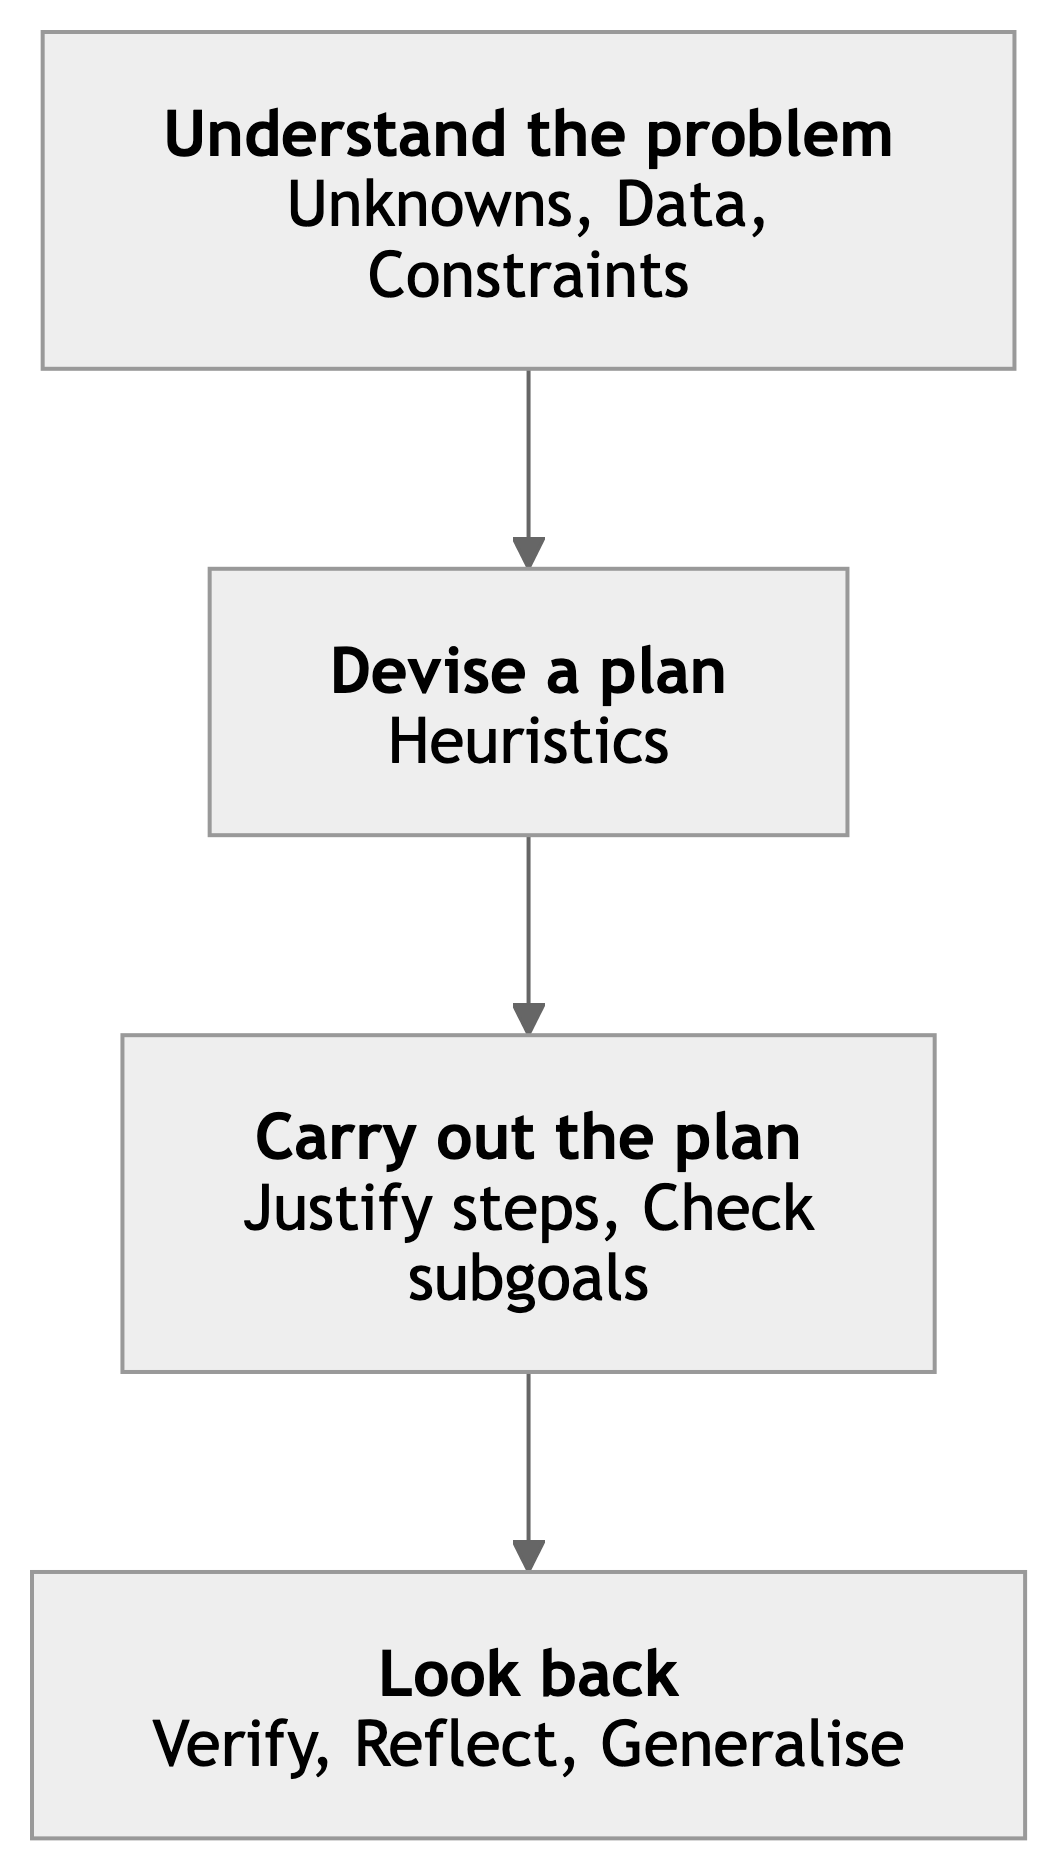
\includegraphics[width=4.26in,height=7.05in]{02-problems_files/figure-latex/mermaid-figure-1.png}

}

\caption{\label{fig-phases}The four phases of problem solving within a
problem solving cycle.}

\end{figure}%

The phases are roughly as follows. First, \textbf{understand the
problem}: identify data/givens, unknowns, and conditions/constraints;
restate it in your own words; sketch, tabulate, or probe small cases.
Next, \textbf{devise a plan} by choosing a route. Possible routes are to
work backward, look for patterns, simplify or specialise, use symmetry
or invariants, introduce an auxiliary object, estimate or bound, change
representation, or reduce to a known problem (we will investigate these
problem solving routes later in Chapter~\ref{sec-heuristics}). Then
\textbf{carry out \emph{your} plan}: execute cleanly, justify each step,
check subgoals, and pivot if a step stalls. Finally, \textbf{look back}:
verify the result, test edge cases, assess efficiency and clarity, and
capture the key idea. The final phase is \emph{essential}. Use the
framework to reflect on what you learned so your future problem solving
gets faster and more reliable.

\section{Phases of problem solving}\label{sec-phases}

Use Table Table~\ref{tbl-phases} as a working checklist and a reflection
guide, not a rigid recipe. As you tackle an open-ended problem, you
might find that you are ``stuck''. First, don't panic! Decide which
phase of the problem solving framework you are in and scan the prompts
in that row. Answering the prompt may lead to a concrete next action.
Reflect on this new action for a few minutes; if it stalls, return to
the table, pick a different prompt, or take a break. Over time, the
prompts will become more familiar and the process of solving an
open-ended problme will be less daunting.

\begin{landscape}

\begin{longtable}[t]{p{0.18\linewidth}p{0.22\linewidth}p{0.30\linewidth}p{0.30\linewidth}}

\caption{\label{tbl-phases}Phases of problem solving, adapted from
(\citeproc{ref-Polya:1945hu}{Pólya 1945, xvi--xvii}).}

\tabularnewline

\toprule
Phase & Purpose & Prompts to ask yourself & Useful tactics\\
\midrule
Understanding the problem & For a problem to find, understand the problem by making the unknown, data, and conditions precise. & What is unknown? What is given or what are the data? What conditions/constraints apply? Can I restate the task in my own words? What do small or extreme cases look like? What diagram/notation will help? & Define symbols. Draw a figure. List constraints. Test tiny cases. Identify edge cases. Rephrase the question. Separate various parts of the condition.\\
Devising a plan & Find the connection between the data and the unknown that provides a path towards a solution. & Have I seen the problem before? Have I seen the same problem in a slightly different form? Do I know a related problem? Do I know a theorem that might be useful? Can I work backward from the goal? Can I simplify/specialise first? What pattern, invariant, or symmetry might apply? Can I introduce an auxiliary element or change representation? Did I use all the data in devising my plan? Did I account for all the conditions? & Heuristics such as analogy; special/edge cases; generalisation; using invariants and symmetry; bounding/estimating; pigeonhole; substitution; set up equations or a new diagram.\\
Carry out your plan & Carry out plan, checking each step! & Would I be able to clearly explain that the step is correct? Can I prove that it is correct? Does each step follow from assumptions or known results? What subgoal can I verify now? If a step fails, which alternative route will I try next? & Justify steps. Prove lemmas. Compute carefully. Frequently take stock (checkpoint). Pivot quickly if a line of attack stalls. Don't panic.\\
Look back & Validate the result and reflect on learning. & Can I check the result? Can you explain your arguments? Does the result meet all conditions? Any counterexamples? Is it complete/optimal? Can I shorten or generalise the solution? Can I derive the result differently? What key idea made it work, and where else could it apply? & Record the central insight. Phases of the framework. Prompts answered. Heuristics used and how.\\
\bottomrule

\end{longtable}

\end{landscape}

\chapter{Heuristics}\label{sec-heuristics}

\begin{quote}
``This principle is so perfectly general that no particular application
of it is possible.'' -- George Pólya
(\citeproc{ref-MacTutor:Polya}{MacTutor 2025a})
\end{quote}

\section{What is a heuristic?}\label{what-is-a-heuristic}

A \emph{heuristic} is a problem-solving device or strategy that provides
a way to seeing or approaching a problem. Choosing a suitable heuristic
often leads us closer to a solution. These strategies are versatile,
applying across a wide range of domains and topics. However, heuristics
alone are not enough to solve a problem; they must be combined with
relevant knowledge and a refined ability to select and deploy
mathematical resources effectively. By explicitly discussing and
reflecting on problem-solving strategies, we aim to bring the use of
heuristics into your conscious awareness. This focus will help you
create connections between different areas of mathematical knowledge and
enhance your reasoning skills. By honing these abilities, you will be
equipped with the tools necessary to become a proficient and literate
problem solver.

\begin{tcolorbox}[enhanced jigsaw, colbacktitle=quarto-callout-warning-color!10!white, left=2mm, colback=white, rightrule=.15mm, toprule=.15mm, bottomrule=.15mm, colframe=quarto-callout-warning-color-frame, bottomtitle=1mm, opacityback=0, toptitle=1mm, titlerule=0mm, coltitle=black, breakable, title=\textcolor{quarto-callout-warning-color}{\faExclamationTriangle}\hspace{0.5em}{Heuristics will not replace shaky mastery of a subject!}, arc=.35mm, opacitybacktitle=0.6, leftrule=.75mm]

``Despite the fact that their application cuts across various
mathematical domains, the successful implementation of heuristic
strategies in any particular domain often depends heavily on the
possession of specific subject matter knowledge.''
(\citeproc{ref-Schoenfeld:1985ps}{Schoenfeld 1985})

\end{tcolorbox}

\section{Compendium of heuristics}\label{compendium-of-heuristics}

Below we include a collection of common heuristics, grouped by theme.
Each of these heuristics should be viewed as a label for a closely
related family of devices. That is, each heuristic in the compendium is
not precise enough to allow for unambiguous interpretation or
application to a particular problem! Key challenges that arise when
trying to apply any of these heuristics is firstly to select
appropriately and second to decompose the heuristic into a targeted
strategy that you can actually execute. Use the prompts to trigger
action.

For each heuristic we have indicated a source: (P) = after Pólya
(\citeproc{ref-Polya:1945hu}{Pólya 1945}); (M) = after Mahajan
(\citeproc{ref-Mahajan:2010ps}{Mahajan 2010}); (MF) = after
(\citeproc{ref-MichalewiczFogel:2004hu}{Michalewicz and Fogel 2004});
(Z) = after (\citeproc{ref-Zeitz:2016ps}{Zeitz 2016}). The list is not
exhaustive.

\subsection*{Variation of the problem}\label{variation-of-the-problem}
\addcontentsline{toc}{subsection}{Variation of the problem}

\begin{tcolorbox}[enhanced jigsaw, colbacktitle=quarto-callout-note-color!10!white, left=2mm, colback=white, rightrule=.15mm, toprule=.15mm, bottomrule=.15mm, colframe=quarto-callout-note-color-frame, bottomtitle=1mm, opacityback=0, toptitle=1mm, titlerule=0mm, coltitle=black, breakable, title={Decomposing and recombining (P, Z)}, arc=.35mm, opacitybacktitle=0.6, leftrule=.75mm]

Break the task into subproblems (lemmas, cases), solve pieces, then
reassemble.

\emph{Prompts}: What minimal subgoal would help? Can I prove a lemma
that reduces the main load?

\end{tcolorbox}

\begin{tcolorbox}[enhanced jigsaw, colbacktitle=quarto-callout-note-color!10!white, left=2mm, colback=white, rightrule=.15mm, toprule=.15mm, bottomrule=.15mm, colframe=quarto-callout-note-color-frame, bottomtitle=1mm, opacityback=0, toptitle=1mm, titlerule=0mm, coltitle=black, breakable, title={Establishing and using subgoals (P, Z)}, arc=.35mm, opacitybacktitle=0.6, leftrule=.75mm]

Name intermediate targets that make progress observable.

\emph{Prompts}: What would I need to show to make the last step trivial?

\end{tcolorbox}

\begin{tcolorbox}[enhanced jigsaw, colbacktitle=quarto-callout-note-color!10!white, left=2mm, colback=white, rightrule=.15mm, toprule=.15mm, bottomrule=.15mm, colframe=quarto-callout-note-color-frame, bottomtitle=1mm, opacityback=0, toptitle=1mm, titlerule=0mm, coltitle=black, breakable, title={Generalisation (P, Z)}, arc=.35mm, opacitybacktitle=0.6, leftrule=.75mm]

Widen the problem to expose structure (a parameter, a family).

\emph{Prompts}: If \(n\) were real/complex/\(d\)-dimensional, what
pattern emerges?

\end{tcolorbox}

\begin{tcolorbox}[enhanced jigsaw, colbacktitle=quarto-callout-note-color!10!white, left=2mm, colback=white, rightrule=.15mm, toprule=.15mm, bottomrule=.15mm, colframe=quarto-callout-note-color-frame, bottomtitle=1mm, opacityback=0, toptitle=1mm, titlerule=0mm, coltitle=black, breakable, title={Specialisation (P, Z)}, arc=.35mm, opacitybacktitle=0.6, leftrule=.75mm]

Test instructive instances (small, extreme, symmetric).

\emph{Prompts}: What happens for \(n = 1, 2, 3\)? For an extreme or
degenerate case?

Note: Trying special cases can suggest both direction and plausibility
of a solution (S).

\end{tcolorbox}

\begin{tcolorbox}[enhanced jigsaw, colbacktitle=quarto-callout-note-color!10!white, left=2mm, colback=white, rightrule=.15mm, toprule=.15mm, bottomrule=.15mm, colframe=quarto-callout-note-color-frame, bottomtitle=1mm, opacityback=0, toptitle=1mm, titlerule=0mm, coltitle=black, breakable, title={Analogy (P, M, Z)}, arc=.35mm, opacitybacktitle=0.6, leftrule=.75mm]

Map the problem to a known cousin and import its method.

\emph{Prompts}: What solved problem has the same backbone (invariant,
recurrence, symmetry)?

\end{tcolorbox}

\subsection*{Auxiliary}\label{auxiliary}
\addcontentsline{toc}{subsection}{Auxiliary}

\begin{tcolorbox}[enhanced jigsaw, colbacktitle=quarto-callout-note-color!10!white, left=2mm, colback=white, rightrule=.15mm, toprule=.15mm, bottomrule=.15mm, colframe=quarto-callout-note-color-frame, bottomtitle=1mm, opacityback=0, toptitle=1mm, titlerule=0mm, coltitle=black, breakable, title={Auxiliary elements (P, Z)}, arc=.35mm, opacitybacktitle=0.6, leftrule=.75mm]

Introduce a helper variable/point/construction (e.g., an extra line in a
diagram, a slack variable).

\emph{Prompts}: What new object would make the relation linear or
symmetric?

\end{tcolorbox}

\begin{tcolorbox}[enhanced jigsaw, colbacktitle=quarto-callout-note-color!10!white, left=2mm, colback=white, rightrule=.15mm, toprule=.15mm, bottomrule=.15mm, colframe=quarto-callout-note-color-frame, bottomtitle=1mm, opacityback=0, toptitle=1mm, titlerule=0mm, coltitle=black, breakable, title={Auxiliary problem (P, Z)}, arc=.35mm, opacitybacktitle=0.6, leftrule=.75mm]

Solve a carefully chosen easier or nearby problem, then adapt.

\emph{Prompts}: What relaxation or stronger statement is tractable?

\end{tcolorbox}

\subsection*{Representation}\label{representation}
\addcontentsline{toc}{subsection}{Representation}

\begin{tcolorbox}[enhanced jigsaw, colbacktitle=quarto-callout-note-color!10!white, left=2mm, colback=white, rightrule=.15mm, toprule=.15mm, bottomrule=.15mm, colframe=quarto-callout-note-color-frame, bottomtitle=1mm, opacityback=0, toptitle=1mm, titlerule=0mm, coltitle=black, breakable, title={Notation (P, Z)}, arc=.35mm, opacitybacktitle=0.6, leftrule=.75mm]

Choose symbols that expose structure (indices, function names,
operators). Rename until the pattern is visible.

\emph{Prompts}: Can I re-index or re-parameterise to simplify sums or
products?

\end{tcolorbox}

\begin{tcolorbox}[enhanced jigsaw, colbacktitle=quarto-callout-note-color!10!white, left=2mm, colback=white, rightrule=.15mm, toprule=.15mm, bottomrule=.15mm, colframe=quarto-callout-note-color-frame, bottomtitle=1mm, opacityback=0, toptitle=1mm, titlerule=0mm, coltitle=black, breakable, title={Figures (P, Z)}, arc=.35mm, opacitybacktitle=0.6, leftrule=.75mm]

Draw to think: diagrams, timelines, tables, state graphs. Iterate the
figure as the plan evolves.

\emph{Prompts}: What picture would let me see the invariant or the
bottleneck?

\end{tcolorbox}

\begin{tcolorbox}[enhanced jigsaw, colbacktitle=quarto-callout-note-color!10!white, left=2mm, colback=white, rightrule=.15mm, toprule=.15mm, bottomrule=.15mm, colframe=quarto-callout-note-color-frame, bottomtitle=1mm, opacityback=0, toptitle=1mm, titlerule=0mm, coltitle=black, breakable, title={Setting up equations (P, Z)}, arc=.35mm, opacitybacktitle=0.6, leftrule=.75mm]

Translate words to algebra/constraints/recurrences. Define variables
cleanly and encode conditions faithfully.

\emph{Prompts}: What are the unknowns, and what relations tie them
together?

\end{tcolorbox}

\subsection*{Verification}\label{verification}
\addcontentsline{toc}{subsection}{Verification}

\begin{tcolorbox}[enhanced jigsaw, colbacktitle=quarto-callout-note-color!10!white, left=2mm, colback=white, rightrule=.15mm, toprule=.15mm, bottomrule=.15mm, colframe=quarto-callout-note-color-frame, bottomtitle=1mm, opacityback=0, toptitle=1mm, titlerule=0mm, coltitle=black, breakable, title={Examine your guess (P, Z)}, arc=.35mm, opacitybacktitle=0.6, leftrule=.75mm]

Conjecture, then interrogate it (``invent then verify''). Try
counterexamples or edge cases; refine if it survives.

\emph{Prompts}: What would falsify my guess quickest?

\end{tcolorbox}

\begin{tcolorbox}[enhanced jigsaw, colbacktitle=quarto-callout-note-color!10!white, left=2mm, colback=white, rightrule=.15mm, toprule=.15mm, bottomrule=.15mm, colframe=quarto-callout-note-color-frame, bottomtitle=1mm, opacityback=0, toptitle=1mm, titlerule=0mm, coltitle=black, breakable, title={Check the result (P, Z)}, arc=.35mm, opacitybacktitle=0.6, leftrule=.75mm]

Verify against all conditions; try alternative derivations; sanity-check
units and orders of magnitude.

\emph{Prompts}: Does this fail for any small or extreme case? Can I
justify uniqueness or optimality?

\end{tcolorbox}

\begin{tcolorbox}[enhanced jigsaw, colbacktitle=quarto-callout-note-color!10!white, left=2mm, colback=white, rightrule=.15mm, toprule=.15mm, bottomrule=.15mm, colframe=quarto-callout-note-color-frame, bottomtitle=1mm, opacityback=0, toptitle=1mm, titlerule=0mm, coltitle=black, breakable, title={Type checking and dimensional analysis (P, M)}, arc=.35mm, opacitybacktitle=0.6, leftrule=.75mm]

Ensure expressions have the right kind: units, dimensions, domains,
monotonicity.

\emph{Prompts}: Do both sides have the same units/type? What scales does
the answer depend on?

\end{tcolorbox}

\subsection*{Inference}\label{inference}
\addcontentsline{toc}{subsection}{Inference}

\begin{tcolorbox}[enhanced jigsaw, colbacktitle=quarto-callout-note-color!10!white, left=2mm, colback=white, rightrule=.15mm, toprule=.15mm, bottomrule=.15mm, colframe=quarto-callout-note-color-frame, bottomtitle=1mm, opacityback=0, toptitle=1mm, titlerule=0mm, coltitle=black, breakable, title={Working backwards (P, Z)}, arc=.35mm, opacitybacktitle=0.6, leftrule=.75mm]

Start from the goal and seek necessary predecessors. Useful for
equations, constructions, and proofs by equivalence.

\emph{Prompts}: If the claim were true, what must also be true one step
earlier?

\end{tcolorbox}

\begin{tcolorbox}[enhanced jigsaw, colbacktitle=quarto-callout-note-color!10!white, left=2mm, colback=white, rightrule=.15mm, toprule=.15mm, bottomrule=.15mm, colframe=quarto-callout-note-color-frame, bottomtitle=1mm, opacityback=0, toptitle=1mm, titlerule=0mm, coltitle=black, breakable, title={Indirect proof (P, Z)}, arc=.35mm, opacitybacktitle=0.6, leftrule=.75mm]

Assume the opposite; derive a contradiction (impossible inequality,
parity clash, minimal counterexample loop).

\emph{Prompts}: What invariant would be violated if the claim were
false?

Note: also called \emph{reductio ad absurdum}.

\end{tcolorbox}

\subsection*{Modern/computational}\label{moderncomputational}
\addcontentsline{toc}{subsection}{Modern/computational}

\begin{tcolorbox}[enhanced jigsaw, colbacktitle=quarto-callout-note-color!10!white, left=2mm, colback=white, rightrule=.15mm, toprule=.15mm, bottomrule=.15mm, colframe=quarto-callout-note-color-frame, bottomtitle=1mm, opacityback=0, toptitle=1mm, titlerule=0mm, coltitle=black, breakable, title={Approximation (M)}, arc=.35mm, opacitybacktitle=0.6, leftrule=.75mm]

Replace an intractable object with a manageable surrogate
(linearisation, asymptotics, bounding, surrogate loss).

\emph{Prompts}: What can I ignore or approximate without changing the
leading behaviour?

\end{tcolorbox}

\begin{tcolorbox}[enhanced jigsaw, colbacktitle=quarto-callout-note-color!10!white, left=2mm, colback=white, rightrule=.15mm, toprule=.15mm, bottomrule=.15mm, colframe=quarto-callout-note-color-frame, bottomtitle=1mm, opacityback=0, toptitle=1mm, titlerule=0mm, coltitle=black, breakable, title={Estimation (M)}, arc=.35mm, opacitybacktitle=0.6, leftrule=.75mm]

Get ballpark numbers (orders of magnitude, back-of-envelope). Use to
choose plans and catch nonsense early.

\emph{Prompts}: What's a plausible scale? Is my result within it?

\end{tcolorbox}

\begin{tcolorbox}[enhanced jigsaw, colbacktitle=quarto-callout-note-color!10!white, left=2mm, colback=white, rightrule=.15mm, toprule=.15mm, bottomrule=.15mm, colframe=quarto-callout-note-color-frame, bottomtitle=1mm, opacityback=0, toptitle=1mm, titlerule=0mm, coltitle=black, breakable, title={Exhaustive search (MF)}, arc=.35mm, opacitybacktitle=0.6, leftrule=.75mm]

Systematically enumerate candidates (with pruning).

\emph{Prompts}: How can I bound the search space? What constraints let
me cut branches?

\end{tcolorbox}

\begin{tcolorbox}[enhanced jigsaw, colbacktitle=quarto-callout-note-color!10!white, left=2mm, colback=white, rightrule=.15mm, toprule=.15mm, bottomrule=.15mm, colframe=quarto-callout-note-color-frame, bottomtitle=1mm, opacityback=0, toptitle=1mm, titlerule=0mm, coltitle=black, breakable, title={Greedy algorithms (MF)}, arc=.35mm, opacitybacktitle=0.6, leftrule=.75mm]

Make the best local choice at each step; accept that it may be
suboptimal globally.

\emph{Prompts}: What local score aligns with the global objective?

\end{tcolorbox}

\begin{tcolorbox}[enhanced jigsaw, colbacktitle=quarto-callout-note-color!10!white, left=2mm, colback=white, rightrule=.15mm, toprule=.15mm, bottomrule=.15mm, colframe=quarto-callout-note-color-frame, bottomtitle=1mm, opacityback=0, toptitle=1mm, titlerule=0mm, coltitle=black, breakable, title={Randomisation and probabilistic methods (MF)}, arc=.35mm, opacitybacktitle=0.6, leftrule=.75mm]

Use randomness to prove existence, estimate quantities, or guide search.

\emph{Prompts}: What random construction has the right expectation? Can
sampling expose the pattern?

\end{tcolorbox}

\begin{tcolorbox}[enhanced jigsaw, colbacktitle=quarto-callout-note-color!10!white, left=2mm, colback=white, rightrule=.15mm, toprule=.15mm, bottomrule=.15mm, colframe=quarto-callout-note-color-frame, bottomtitle=1mm, opacityback=0, toptitle=1mm, titlerule=0mm, coltitle=black, breakable, title={Neural Networks / learned heuristics (MF)}, arc=.35mm, opacitybacktitle=0.6, leftrule=.75mm]

Use a trained model to guide search and propose candidates or rank moves
(proof search, construction hints).

\emph{Prompts}: What features or examples could a model learn from? How
do I verify its suggestions?

\end{tcolorbox}

\chapter{Attitudes}\label{sec-attitudes}

\begin{quote}
``Many people who have not studied mathematics confuse it with
arithmetic and consider it a dry and fruitless science. In reality,
however, it is a science which requires a great amount of imagination.''
-- Sofia Kovalevskaya (\citeproc{ref-MacTutor:Kovalevskaya}{MacTutor
2025b})
\end{quote}

Effective problem solvers masterfully balance curiosity with discipline.
They begin by probing, playing, and hypothesizing, then move on to
justifying, checking, and reflecting on their findings. According to
Pólya, true progress originates from cycling through the four
problem-solving phases, maintaining a keen awareness of one's actions,
and a readiness to adapt when new evidence arises
(\citeproc{ref-Polya:1945hu}{Pólya 1945}). When progress stalls, adept
problem solvers pivot swiftly and consistently take time to ``look
back'' at their process.

\section{Selecting and pursuing an
approach}\label{selecting-and-pursuing-an-approach}

Begin by matching structure to strategy. Let the problem's cues choose
the method: a recurrence invites induction; symmetry points toward
invariants; a geometric flavour asks for a diagram and auxiliary
elements; unruly numbers suggest estimation or approximation.

Then commit to a strategy, but keep your course of action time-bound.
Choose one plan and pursue it deliberately for a few minutes. Set a
concrete checkpoint in advance so the decision to switch is not
emotional or driven by frustration (``If I cannot determine the number
of cases in twenty minutes, I will try another approach.'').

Finally, watch for traction. You are on the right track if relations
clarify, expressions simplify, or the number of cases shrinks. If
instead the algebra gets tedious, cases proliferate, or your reasoning
seems circular: stop, reframe the problem, and select a different
strategy.

\section{Still stuck?}\label{still-stuck}

\begin{tcolorbox}[enhanced jigsaw, colbacktitle=quarto-callout-important-color!10!white, left=2mm, colback=white, rightrule=.15mm, toprule=.15mm, bottomrule=.15mm, colframe=quarto-callout-important-color-frame, bottomtitle=1mm, opacityback=0, toptitle=1mm, titlerule=0mm, coltitle=black, breakable, title=\textcolor{quarto-callout-important-color}{\faExclamation}\hspace{0.5em}{Try answering these questions:}, arc=.35mm, opacitybacktitle=0.6, leftrule=.75mm]

\begin{itemize}
\tightlist
\item
  What exactly are you doing? Can you describe it precisely?
\item
  Why are you doing it? How does it fit into the solution?
\item
  How does it help you? What will you do with the outcome when you
  obtain it?
\end{itemize}

(see \citeproc{ref-Schoenfeld:1985ps}{Schoenfeld 1985}).

\end{tcolorbox}

\chapter*{References}\label{references}
\addcontentsline{toc}{chapter}{References}

\markboth{References}{References}

\begingroup
\raggedright

\phantomsection\label{refs}
\begin{CSLReferences}{1}{0}
\bibitem[\citeproctext]{ref-Halmos:1980ps}
Halmos, P. R. 1980. {``The Heart of Mathematics.''} \emph{The American
Mathematical Monthly} 87 (7): 519--24.
\url{https://doi.org/10.2307/2321415}.

\bibitem[\citeproctext]{ref-MacTutor:Polya}
MacTutor. 2025a. {``Quotation by George p{ó}lya.''} University of St
Andrews. 2025.
\url{https://mathshistory.st-andrews.ac.uk/Biographies/Polya/quotations}.

\bibitem[\citeproctext]{ref-MacTutor:Kovalevskaya}
---------. 2025b. {``Quotation by Sofia Kovalevskaya.''} University of
St Andrews. 2025.
\url{https://mathshistory.st-andrews.ac.uk/Biographies/Kovalevskaya/quotations}.

\bibitem[\citeproctext]{ref-Mahajan:2010ps}
Mahajan, Sanjoy. 2010. \emph{Street-Fighting Mathematics: The Art of
Educated Guessing and Opportunistic Problem Solving}. Cambridge, MA: The
MIT Press. \url{https://doi.org/10.7551/mitpress/7728.001.0001}.

\bibitem[\citeproctext]{ref-MichalewiczFogel:2004hu}
Michalewicz, Zbigniew, and David B. Fogel. 2004. \emph{{How to Solve It:
Modern Heuristics}}. 2nd ed. Berlin, Heidelberg: Springer.
\url{https://doi.org/10.1007/978-3-662-07807-5}.

\bibitem[\citeproctext]{ref-OED:1989ps}
\emph{Oxford English Dictionary}. 1989. 2nd ed. Oxford: Oxford
University Press.

\bibitem[\citeproctext]{ref-Polya:1945hu}
Pólya, George. 1945. \emph{{How to Solve It}}. Princeton, NJ: Princeton
University Press.

\bibitem[\citeproctext]{ref-Polya:1954oi}
---------. 1954a. \emph{Mathematics and Plausible Reasoning, Volume 1:
Induction and Analogy in Mathematics}. Princeton, NJ: Princeton
University Press.

\bibitem[\citeproctext]{ref-Polya:1954ii}
---------. 1954b. \emph{Mathematics and Plausible Reasoning, Volume 2:
Logic, Symbolic and Mathematical}. Princeton, NJ: Princeton University
Press.

\bibitem[\citeproctext]{ref-Schoenfeld:1985ps}
Schoenfeld, Alan H. 1985. \emph{Mathematical Problem Solving}. Orlando,
FL: Academic Press. \url{https://doi.org/10.1016/C2013-0-05012-8}.

\bibitem[\citeproctext]{ref-Zeitz:2016ps}
Zeitz, Paul. 2016. \emph{The Art and Craft of Problem Solving}. 3rd ed.
Hoboken, NJ: Wiley.

\end{CSLReferences}

\endgroup

\part{Professional Skills}




\end{document}
